\setauthor{Antonio Kuvac}

Die erste und auch längste Phase dieses Projekts war die Planung. 
In der Planungsphase wurden verschiedenste Kreativitätstechniken angewandt und Dokumente, die für die Planung unerlässlich sind, erstellt.

\section{Projektpartnermeetings}
\setauthor{Antonio Kuvac}

Der Grundstein für diese Arbeit waren die abgehaltenen Meetings mit dem Projektpartner dieses Projekts. Bei den ersten Meetings wurde definiert, was die App können muss und wie die App auszusehen hat
um Missverständnisse im voraus zu behandeln und um sich ein Bild darüber zu machen, welche Anforderungen das Projekt hat und welche Herausforderungen zu bewältigen sind. 
Mit diesen Meetings wurde der Projektpartner auch auf aktuellen Stand gehalten und auftretende Probleme und Anmerkungen, 
die bei der Arbeit am Projekt entstanden sind, wurden besprochen und abgehandelt.

\section{Use-Case Diagramm}
\setauthor{Antonio Kuvac}

Ein Use Case Diagramm oder auch Anwendungsfalldiagramm ist ein Diagramm von Anwendungsfällen und ihren Beziehungen zu ihrer Umgebung und zu anderen Anwendungsfällen. 
Damit beschreibt es, welche Funktionen und Dienste ein System für einen Anwender bereitstellt.
Mit einem Use Case Diagramm werden weder die Abläufe des Systems beschrieben, 
noch die Reihenfolge der Funktionen oder Dienste dargestellt. 
Ein Anwendungsfalldiagramm visualisiert lediglich die Zusammenhänge zwischen einer Menge von Use Cases und den involvierten Akteuren. Damit eignet es sich sehr gut zur Anforderungsanalyse, also zur Ermittlung oder Verfeinerung von Anforderungen.
\pagebreak
\subsection{Elemente im Use-Case Diagramm}

Folgende Elemente sind in einem Use-Case Diagramm üblicherweise enthalten:
\begin{itemize}
    \item System: Das System ist an sich kein logisches Modellelement, sondern grenzt den Kontext ab. Das System wird durch eine Box im Diagramm dargestellt, in dem das System seine Funktionen und Dienste zur Verfügung stellt.
    \item Akteur: Der Akteur befindet sich außerhalb des Systems. Er wird als Strichmännchen gezeichnet und kann eine konkrete Person aber auch ein abstraktes Element wie zum Beispiel ein Sensor sein. Wird ein Akteur definiert, muss dieser auch immer mit mindestens einem Use Case in Verbindung stehen.
    \item Anwendungsfall: Ein Anwendungsfall wird meistens als Ellipse visualisiert. Ein Diagramm kann mehrere Anwendungsfälle besitzen. Ist ein Use Case nur durch andere Anwendungsfälle ausführbar, wird er als abstrakt bezeichnet.
    \item Beziehungen: Zwischen Akteuren und Anwendungsfällen oder zwischen Anwendungsfällen selbst bestehen Beziehungen. Sie werden meistens als Linien oder Pfeile zwischen den jeweiligen Objekten eingezeichnet.
    \item Notizen: Mit Notizen lassen sich Informationen hinzufügen, um das Verständnis zu erhöhen. Sie werden mit einem Rechteck dargestellt, dessen obere rechte Ecke eingeknickt ist. Eine gestichelte Linie verbindet die Notiz mit dem zu erklärenden Element.
    
    \end{itemize}
    \pagebreak
    \subsection{Verwendung des Use-Case Diagramms in der Diplomarbeit}

    Das Use Case Diagramm wurde verwendet um Klarheit über die Funktionen und den Akteuren zu schaffen und für Vergewisserung zu sorgen, dass keine wichtigen Verbindungen vergessen wurden.
    Am Ende der Planungsphase angelangt sieht das Use-Case Diagramm wie folgt aus:

    \begin{figure}[H]
        \centering
        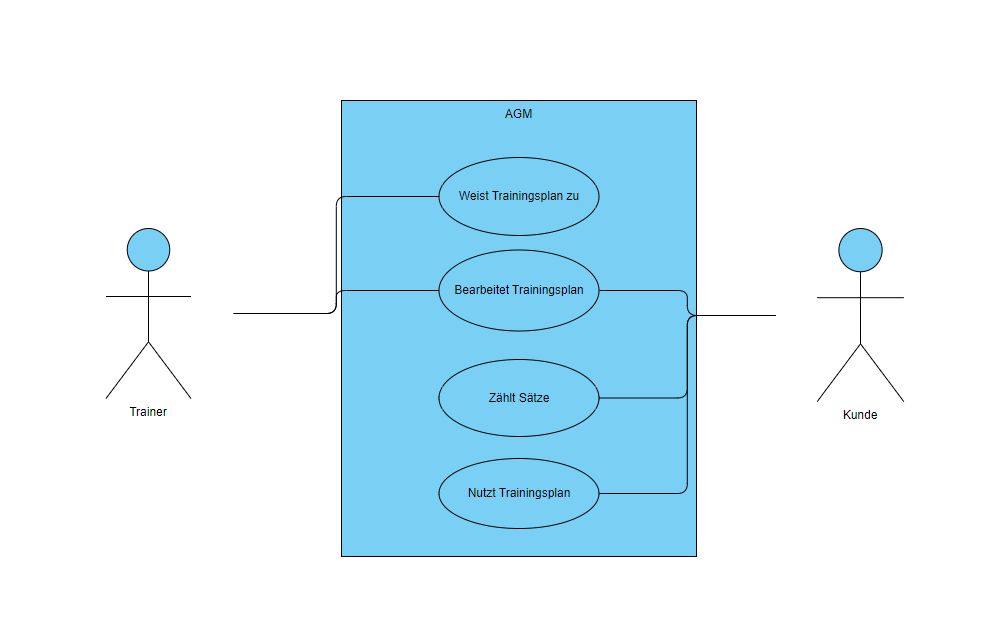
\includegraphics[scale=0.6]{pics/Use Case Diagramm.png}
        \caption{Use-Case Diagramm}
    \end{figure}


    \section{Entity Relationship Diagram - ERD}
    \setauthor{Antonio Kuvac}

    Ein ERD ist ein Diagramm der Beziehungen (Relationship) zwischen Entitäten (Entity) in einem Datenbankschema darstellt. 
    Es wird verwendet, um das Design einer Datenbank zu modellieren und darzustellen und wie Daten in der Datenbank organisiert und miteinander verbunden sind.

    \pagebreak

    \subsection{Komponenten eines ERDs}

    Üblicherweise bestehen ERD-Diagramme aus drei Hauptkomponenten, und zwar aus Entitäten, Attributen und Beziehungen.

    \begin{itemize}
        \item Entitäten: Eine Entität repräsentiert eine Klasse von Objekten, die bestimmte Eigenschaften oder Attribute gemeinsam haben. Ein Beispiel für eine Entität wäre zum Beispiel ein Kunde der als Attribute einen Namen und eine Wohnadresse hat. Entitäten werden meistens als Rechtecke dargestellt
        \item Attribute: Attribute sind die Eigenschaften, die die Entitäten beschreiben, wie beispielsweise der Name eines Kunden oder die Menge eines Produkts. Attribute werden meistens durch Ellipsen dargestellt können aber auch in der Entität selbst drinnen stehen.
        \item Beziehungen: Beziehungen beschreiben die Art und Weise, wie Entitäten miteinander in Verbindung stehen. 
        Man unterscheidet zwischen drei Arten von Beziehungen. Die erste ist One-to-One.  Diese Beziehung tritt auf, wenn jeder Datensatz in der ersten Tabelle nur einen entsprechenden Datensatz in der zweiten Tabelle hat und umgekehrt. Ein Beispiel dazu wäre eine Person und sein Reisepass, denn jede Person hat nur einen Reisepass und ein Reisepass gehört nur zu einer Person.
        Die zweite Art ist One-to-Many. Diese Beziehung tritt auf, wenn ein Datensatz in der ersten Tabelle mehrere Datensätze in der zweiten Tabelle hat. Ein Beispiel dafür ist eine Mutter die mehrere Kinder hat, aber jedes Kind hat nur eine leibliche Mutter.
        Die Letzte Art von Beziehung ist Many-to-Many.Diese Beziehung tritt auf, wenn ein Datensatz in der ersten Tabelle mehrere Datensätze in der zweiten Tabelle hat, aber auch umgekehrt. Ein Beispiel für diese Beziehung ist ein Student der mehrere Kurse hat und ein Kurs der mehrere Studenten hat.

        \end{itemize}

        \pagebreak

    \subsection{Verwendung des Entity Relationship Diagrams in der Diplomarbeit}

    Um eine funktionierende Datenbank für das Backend zu gewährleisten wurde in Zusammenarbeit mit den Mitgliedern vom Projekt AberGym  mithilfe eines ERDs eine Datenbankstruktur erstellt die sowohl für die Anforderungen von AberGym als auch für die Anforderungen von AberGymMobile angepasst ist.

    \begin{figure}[H]
        \centering
        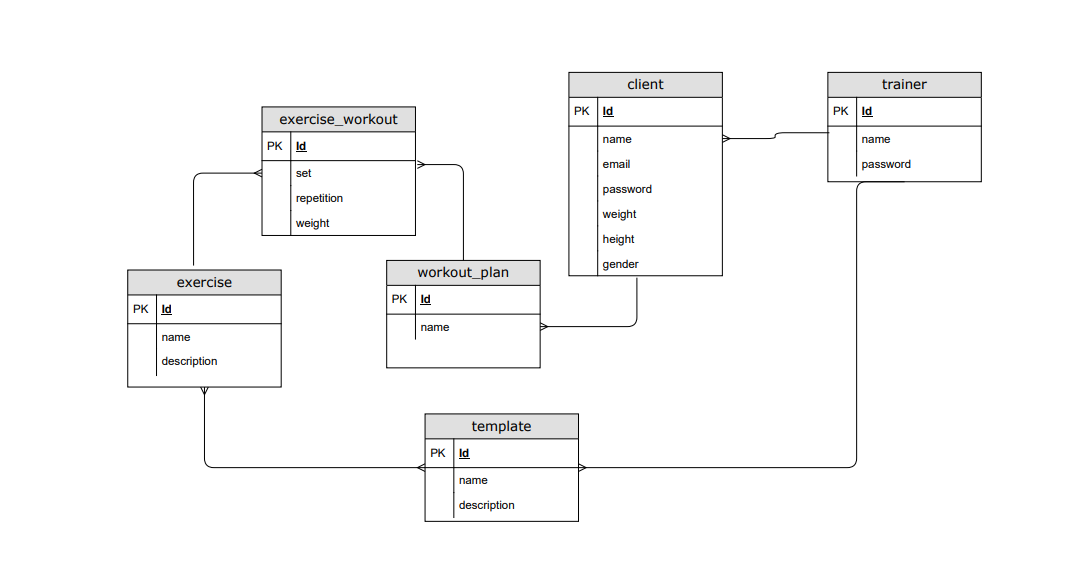
\includegraphics[scale=0.6]{pics/erd plantuml.png}
        \caption{ERD Diagramm in PlantUml}
    \end{figure}

    \subsection{PlantUml}
    PlantUML ist ein Open-Source-Tool zur Erstellung von UML-Diagrammen, das dabei unterstützt, Software-Architekturen, Systemdesigns und Prozessabläufe auf einfache Weise zu visualisieren. Es verwendet eine textbasierte Syntax, um Diagramme zu erstellen, die leicht verständlich, modifizierbar und in verschiedenen Formaten exportierbar sind. In diesem Text werden die wichtigsten Merkmale von PlantUML, seine Anwendungsbereiche sowie einige nützliche Ressourcen vorgestellt.

    \pagebreak
    \section{Design Thinking}
    \setauthor{Antonio Kuvac}


    Design Thinking ist eine innovative Kreativitätstechnik, die in den letzten Jahren immer mehr an Bedeutung gewonnen hat. 
    Diese Methode verbindet kreative und analytische Ansätze, um komplexe Probleme zu lösen und innovative Lösungen zu entwickeln. 
    Design Thinking fördert dabei ein tiefes Verständnis für die Bedürfnisse der Nutzer*innen und stellt diese in den Mittelpunkt des Entwicklungsprozesses. 

   
    \subsection{Phasen des Design Thinking}

    Der Design-Thinking-Prozess besteht aus mehreren Phasen, die iterativ und flexibel durchlaufen werden. Diese Phasen sind:

    \begin{itemize}
        \item \textbf{Verstehen:} In dieser Phase geht es darum, das Problem, die Herausforderung oder den Kontext zu erfassen und ein tiefes Verständnis für die Bedürfnisse der Nutzer*innen zu entwickeln.
        \item \textbf{Beobachten:} Durch direkte Beobachtungen, Interviews und andere qualitative Methoden Informationen und Empathie für die Zielgruppe sammeln.
        \item \textbf{Sichten:} Die gesammelten Informationen werden analysiert, um Muster und Zusammenhänge zu erkennen. Hier werden auch Problemstellungen und Fragestellungen definiert.
        \item \textbf{Ideenfindung:} In dieser Phase werden verschiedene Kreativitätstechniken eingesetzt, um möglichst viele und vielfältige Ideen zu generieren.
        \item \textbf{Prototyping:} Die entwickelten Ideen werden in Form von einfachen und kostengünstigen Prototypen umgesetzt, um sie anschließend testen zu können.
        \item \textbf{Testen:} Die Prototypen werden mit der Zielgruppe getestet, um Feedback zu erhalten und die Lösungen kontinuierlich zu verbessern.
    \end{itemize}
    

    \subsection{Verwendung von Design Thinking in der Diplomarbeit}
    Design Thinking wurde während der Planungsphase und darüber hinaus kontinuierlich verwendet. 
    Durch häufige Meetings mit dem Betreuer und dem Projektpartner dieser Diplomarbeit haben Ideen und die Prototypen (Mockups) permanent Feedback erhalten und wurden dementsprechend angepasst und verbessert.

    \section{Brain Storming}
    \setauthor{Antonio Kuvac}

    Brainstorming ist eine weit verbreitete und populäre Kreativitätstechnik, die darauf abzielt, eine Vielzahl von Ideen in kurzer Zeit zu generieren.

    \subsection{Prinzipien von Brainstorming}
    Das Brainstorming basiert auf einigen grundlegenden Prinzipien, die darauf abzielen, die kreative Zusammenarbeit zu fördern und die Entstehung neuer Ideen zu begünstigen. Zu diesen Prinzipien gehören:

    \begin{itemize}
        \item \textbf{Keine Kritik:} Während der Brainstorming-Sitzung sollte jegliche Kritik und Bewertung von Ideen vermieden werden.
        \item \textbf{Quantität geht vor Qualität:} In der Ideengenerierungsphase des Brainstormings ist das Hauptziel, möglichst viele Ideen zu sammeln, unabhängig von ihrer Qualität. Die Auswahl und Bewertung der Ideen erfolgt in einem späteren Schritt.
        \item \textbf{Kombination und Verbesserung von Ideen:} Man wird ermutigt auf bereits geäußerte Ideen aufzubauen und sie zu verbinden oder zu verbessern.
        \item \textbf{Freies Denken:} Brainstorming ist auf unkonventionelle und unerwartete Ideen ausgelegt um keine Ideen als unnötig einzustufen.
    \end{itemize}

    \subsection{Verwendung von Brainstorming in der Diplomarbeit}
    Nach jedem Meeting wurde Brainstorming angewandt um auf alle möglichen Ideen zu kommen. Wenn sich auf etwas geeinigt wurde, wurde es in die Tat umgesetzt, um Feedback dafür zu bekommen.

 \pagebreak

    \section{Kopfstand Methode}
    Die Kopfstand-Methode, ist eine Kreativitätstechnik, die darauf abzielt, sich anstatt direkt auf die Lösung eines Problems zu konzentrieren,  Probleme aus einer negativen Perspektive zu betrachten.

    \begin{itemize}
        \item \textbf{Problemumkehr}: Das ursprüngliche Problem oder die Fragestellung wird in ihr Gegenteil umgeformt, um eine neue Perspektive zu gewinnen.
        
        \item \textbf{Ideengenerierung}: Es werden Ideen entwickelt, die auf die umgekehrte Problemstellung oder Fragestellung abzielen, und konzentrieren sich dabei auf die negativen Aspekte des Themas.
        
        \item \textbf{Umkehr der Lösungsansätze}: Die negativen Ideen werden zurück in positive Lösungsansätze umgewandelt.
        
        \item \textbf{Bewertung und Auswahl}: Die entwickelten Ideen und Lösungsansätze werden hinsichtlich ihrer Anwendbarkeit, Machbarkeit und Relevanz bewertet. Die vielversprechendsten Lösungen können dann weiter verfeinert und in die Praxis umgesetzt werden.
        \end{itemize}

        \subsection{Verwendung der Kopfstand Methode in der Diplomarbeit}
        Durch eine Kombination von anderen Kreativitätstechniken kamen immer Gedanken von Problemen wo sich die frage stellte , welche Probleme man mit gewissen Vorangehensweisen hätte. Somit wurde im Laufe der Planung mit der Kopfstand Methode abgewägt was in naher Zukunft an Problemen bereiten könnte und wie mit diesen Problemen umgegangen wird.  


\newpage
\section{Mockups}
\setauthor{Antonio Peric}  
Im Rahmen des Entwicklungsprozesses unserer mobilen Anwendung haben wir vier verschiedene Mockups erstellt, um das beste Design für die Nutzer*innen zu ermitteln und es optimal an die Bedürfnisse verschiedener Zielgruppen anzupassen. Die Gestaltung dieser Mockups berücksichtigt sowohl ästhetische als auch funktionale Aspekte, um eine ansprechende und effiziente Benutzeroberfläche zu schaffen, die den unterschiedlichen Anforderungen der*die Nutzer*innen gerecht wird.
\newline
\newline
Die vier Mockups wurden sorgfältig entworfen und auf Basis von Designprinzipien und Benutzeranforderungen entwickelt, um sicherzustellen, dass sie alle relevanten Funktionen und Interaktionen der Anwendung abbilden. Dabei wurde darauf geachtet, unterschiedliche Designansätze und Interaktionsmöglichkeiten zu berücksichtigen, um ein breites Spektrum an Nutzerpräferenzen abzudecken.
\newline
\newline
Nach einer umfassenden Analyse und Bewertung der vier Mockups haben unser Berater und Partner das vierte Mockup als das am besten geeignete Design ausgewählt. Dieses Design wurde aufgrund seiner benutzerfreundlichen Gestaltung, der klaren Struktur und der ansprechenden visuellen Elemente bevorzugt. Zudem wurde es als am ehesten in der Lage erachtet, die Bedürfnisse und Anforderungen der verschiedenen Zielgruppen zu erfüllen.

\newpage
Beim Öffnen der mobilen Anwendung gelangen die Nutzer*innen zunächst in den Log-in-Bereich (\hyperref[fig:log1]{siehe Abbildung 1}, \hyperref[fig:log2]{siehe Abbildung 2}). Hier besteht die Möglichkeit, sich mithilfe eines QR-Codes oder NFC-Technologie schnell und unkompliziert einzuloggen. Durch die Integration dieser modernen und benutzerfreundlichen Authentifizierungsmethoden wird der Zugang zur Anwendung für die Nutzer*innen erleichtert und die Sicherheit der persönlichen Daten gewährleistet.

\begin{figure}[!htb]
    \centering
    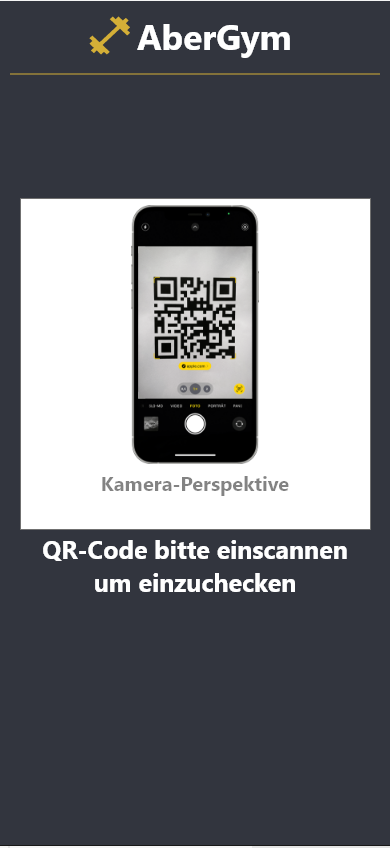
\includegraphics[width=0.35\textwidth]{pics/log1.png}
    \caption{Mockup 1 | Log-in-Bereich der mobilen Anwendung}
    \label{fig:log1}
\end{figure}
\begin{figure}[!htb]
    \centering
    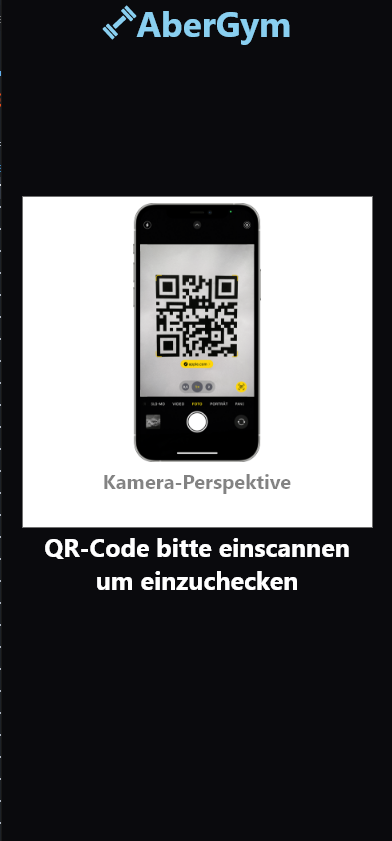
\includegraphics[width=0.35\textwidth]{pics/log2.png}
    \caption{Mockup 2 | Log-in-Bereich der mobilen Anwendung}
    \label{fig:log2}
\end{figure}
\FloatBarrier

Nach erfolgreichem Einloggen in die mobile Anwendung werden die Nutzer*innen automatisch zum heutigen Trainingsplan weitergeleitet. Dort besteht die Möglichkeit, den Trainingsplan jederzeit durch Berührung der Touchfläche {``Trainingsplan starten''} zu starten. Diese benutzerfreundliche Gestaltung ermöglicht einen schnellen Zugriff auf die wichtigsten Funktionen und erleichtert den Einstieg in das Training.
\newline
\newline
In der unteren Leiste, die in \hyperref[fig:main3]{Abbildung 3} und \hyperref[fig:main4]{siehe Abbildung 4} dargestellt ist, können die Nutzer*innen bequem zwischen dem letzten und dem heutigen Trainingsplan navigieren. Diese Funktion erleichtert den Zugriff auf vergangene und aktuelle Trainingspläne und bietet den Nutzer*innen eine flexible Möglichkeit, ihre Trainingshistorie und Fortschritte einzusehen und zu verwalten.

\begin{figure}[!htb]
    \centering
    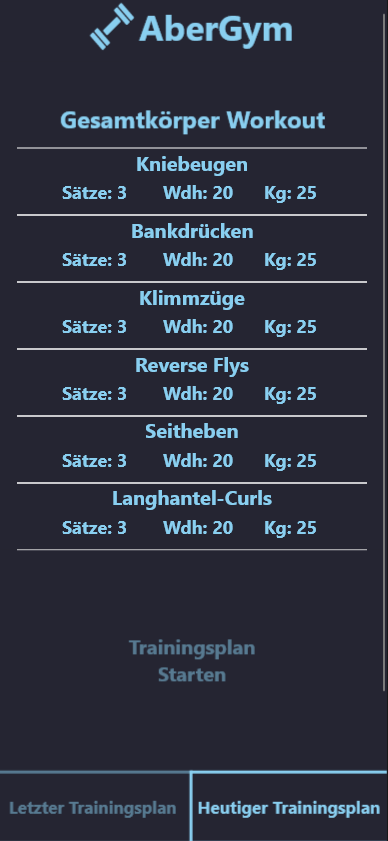
\includegraphics[width=0.35\textwidth]{pics/main3.png}
    \caption{Mockup 3 | Hauptbereich der mobilen Anwendung}
    \label{fig:main3}
\end{figure}
\begin{figure}[!htb]
    \centering
    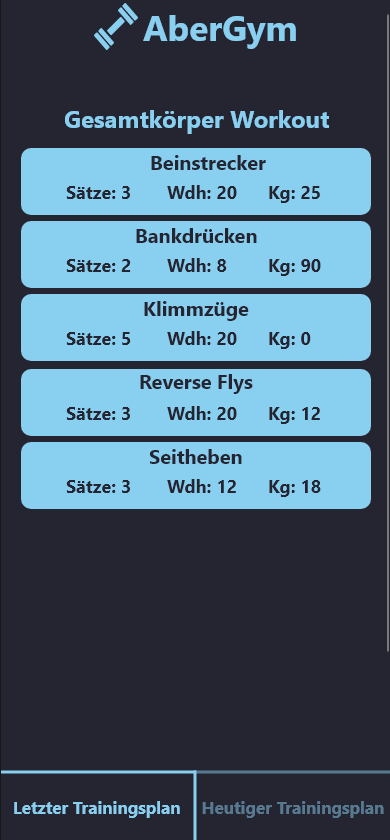
\includegraphics[width=0.35\textwidth]{pics/main4.png}
    \caption{Mockup 4 | Hauptbereich der mobilen Anwendung}
    \label{fig:main4}
\end{figure}
\FloatBarrier

Sobald die Nutzer*innen die Touchfläche {``Trainingsplan starten''} betätigen, wird der heutige Trainingsplan auf einer neuen Seite geöffnet und in einer To-Do-Ansicht präsentiert. In dieser Ansicht können die Nutzer*innen eine beliebige Übung auswählen und durchgehen. Zudem besteht die Möglichkeit, eine Übung zu bearbeiten, indem die Nutzer*innen die gewünschte Übung längere Zeit gedrückt halten. Diese flexible und benutzerfreundliche Gestaltung ermöglicht es den Nutzer*innen, ihren Trainingsplan individuell anzupassen und effizient durchzuarbeiten (\hyperref[fig:todolist1]{siehe Abbildung 5}, \hyperref[fig:todolist2]{siehe Abbildung 6}, \hyperref[fig:todolist3]{siehe Abbildung 7}, \hyperref[fig:todolist4]{siehe Abbildung 8}).

\begin{figure}[!htb]
    \centering
    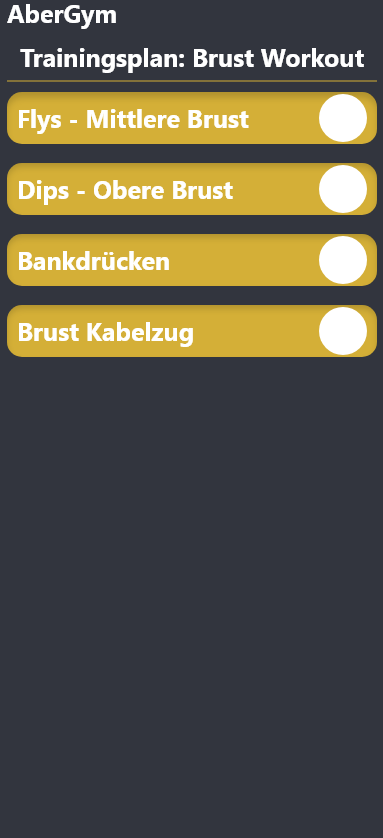
\includegraphics[width=0.35\textwidth]{pics/todolist1.png}
    \caption{Mockup 1 | To-Do-Bereich der mobilen Anwendung}
    \label{fig:todolist1}
\end{figure}
\begin{figure}[!htb]
    \centering
    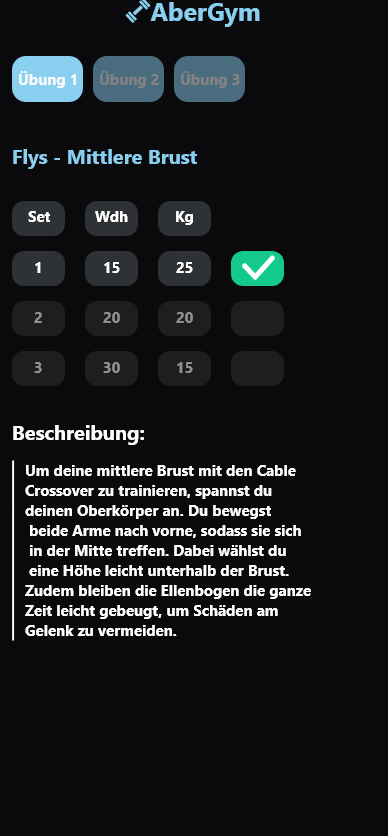
\includegraphics[width=0.35\textwidth]{pics/todolist2.png}
    \caption{Mockup 2 | To-Do-Bereich der mobilen Anwendung}
    \label{fig:todolist2}
\end{figure}
\begin{figure}[!htb]
    \centering
    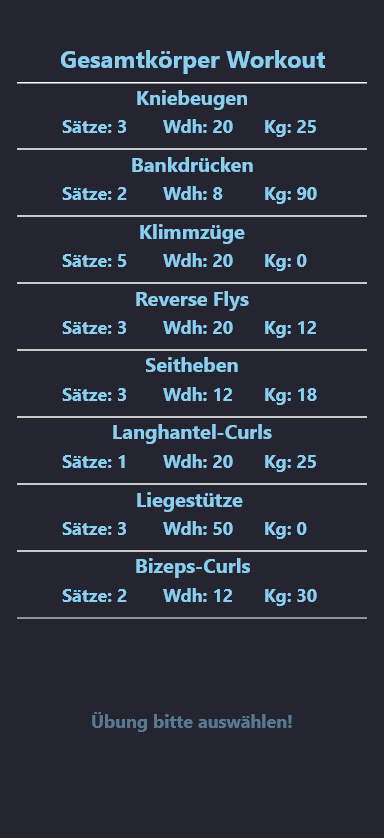
\includegraphics[width=0.35\textwidth]{pics/todolist3.png}
    \caption{Mockup 3 | To-Do-Bereich der mobilen Anwendung}
    \label{fig:todolist3}
\end{figure}
\begin{figure}[!htb]
    \centering
    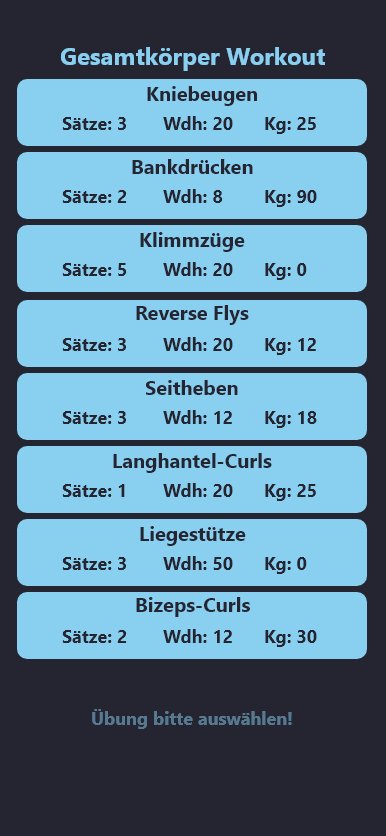
\includegraphics[width=0.35\textwidth]{pics/todolist4.png}
    \caption{Mockup 4 | To-Do-Bereich der mobilen Anwendung}
    \label{fig:todolist4}
\end{figure}
\FloatBarrier

Wenn die Nutzer*innen eine Übung auswählen, wird die entsprechende Übungsinformation erneut angezeigt. In jedem Mockup ist ein Zähler integriert, der bei Berührung des Bildschirms erhöht wird. Der gesamte Bildschirm dient als Druckfläche, um die Bedienung auch für Nutzer*innen mit Handschuhen zu erleichtern, da das Drücken von kleinen Buttons in solchen Situationen schwierig sein kann.
\newline
\newline
Sobald der Zähler den gleichen Wert wie die Satzanzahl der Übung erreicht hat, werden die Nutzer*innen automatisch zur To-Do-Ansicht zurückgeleitet. Die abgeschlossene Übung wird dann grau markiert und ans Ende der Liste verschoben. Dieses intuitive Design ermöglicht es den Nutzer*innen, ihren Fortschritt im Trainingsplan einfach nachzuvollziehen und sich auf die verbleibenden Übungen zu konzentrieren (\hyperref[fig:count1]{siehe Abbildung 9}, \hyperref[fig:todolist2]{siehe Abbildung 6}, \hyperref[fig:count3]{siehe Abbildung 11}, \hyperref[fig:count4]{siehe Abbildung 12}).

\begin{figure}[!htb]
    \centering
    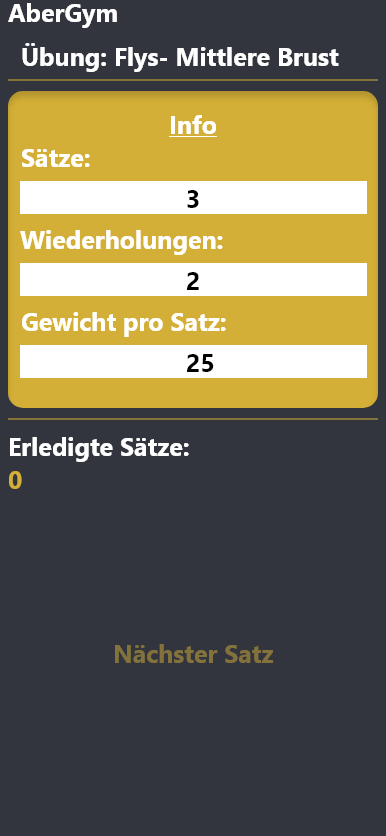
\includegraphics[width=0.35\textwidth]{pics/count1.png}
    \caption{Mockup 1 | Zähl-Bereich der mobilen Anwendung}
    \label{fig:count1}
\end{figure}
\begin{figure}[!htb]
    \centering
    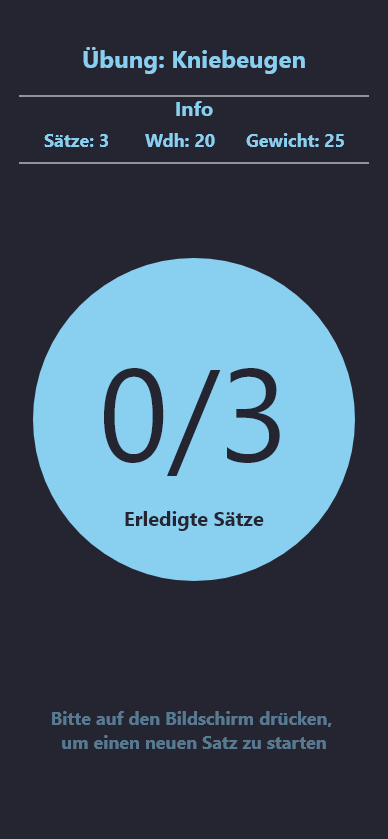
\includegraphics[width=0.35\textwidth]{pics/count3.png}
    \caption{Mockup 3 | Zähl-Bereich der mobilen Anwendung}
    \label{fig:count3}
\end{figure}
\begin{figure}[!htb]
    \centering
    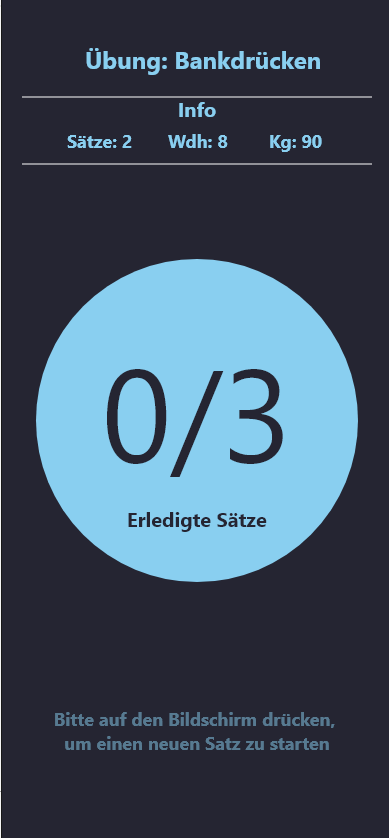
\includegraphics[width=0.35\textwidth]{pics/count4.png}
    \caption{Mockup 4 | Zähl-Bereich der mobilen Anwendung}
    \label{fig:count4}
\end{figure}
\FloatBarrier

Sobald die Nutzer*innen alle Übungen abgeschlossen haben, werden sie zur Hauptseite zurückgeleitet, auf der sie die vorgenommenen Änderungen während der Durchführung des Trainingsplans einsehen können. Der aktualisierte Trainingsplan, der die neuen Werte der jeweils bearbeiteten Übungen enthält, wird unter der Navigation "Heutiger Trainingsplan" angezeigt. Die Nutze*rinnen können den überarbeiteten Trainingsplan erneut durcharbeiten, indem sie die Touchfläche {``Trainingsplan starten''} betätigen.
\newline
\newline
In der Navigation "Letzter Trainingsplan" wird hingegen der ursprüngliche Trainingsplan mit den alten Daten der jeweiligen bearbeiteten Übungen dargestellt. Dieser kann jedoch nicht erneut gestartet werden. Diese Funktion ermöglicht den Nutzer*innen, die Fortschritte und Veränderungen im Trainingsplan nachzuvollziehen und die Entwicklung ihrer Trainingsergebnisse im Zeitverlauf zu verfolgen (\hyperref[fig:finished3]{siehe Abbildung 13}, \hyperref[fig:finished4]{siehe Abbildung 14}).

\begin{figure}[!htb]
    \centering
    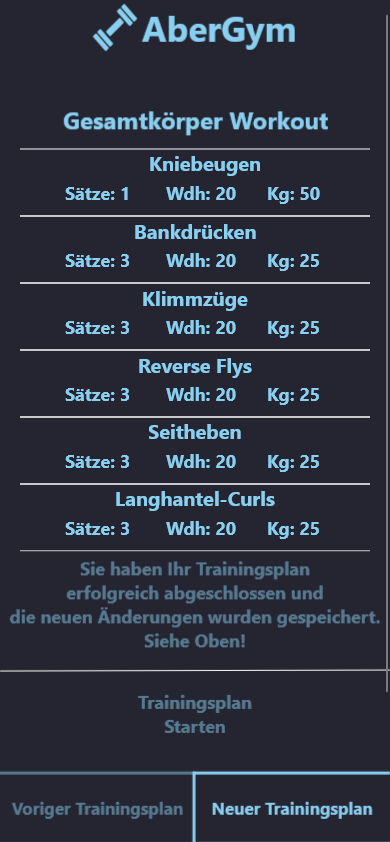
\includegraphics[width=0.35\textwidth]{pics/finished3.png}
    \caption{Mockup 3 | Hauptbereich nach der Durcharbeitung des Trainingplans}
    \label{fig:finished3}
\end{figure}
\begin{figure}[!htb]
    \centering
    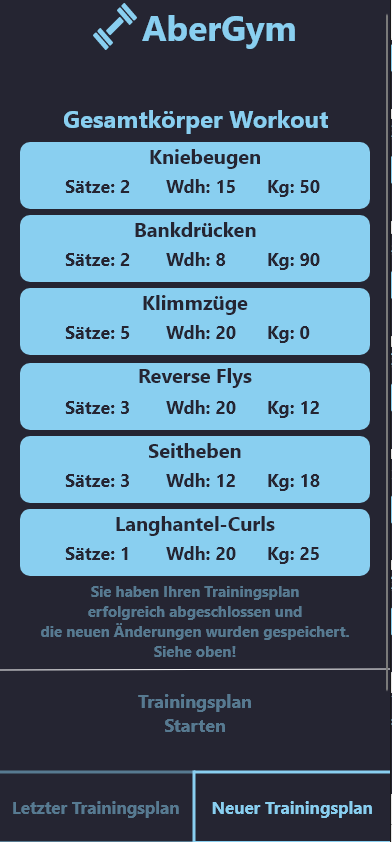
\includegraphics[width=0.35\textwidth]{pics/finished4.png}
    \caption{Mockup 4 | Hauptbereich nach der Durcharbeitung des Trainingplans}
    \label{fig:finished4}
\end{figure}
\FloatBarrier

Obwohl das Mockup 4 ursprünglich ausgewählt wurde, wurde während des Entwicklungsprozesses das Design weiter angepasst, optimiert und verschönert. Diese Änderungen wurden vorgenommen, um den Nutzer*innen die Navigation innerhalb der App zu erleichtern und ihnen dabei zu helfen, sich besser zurechtzufinden. Durch diese Designanpassungen wurde eine benutzerfreundliche und ansprechende Oberfläche geschaffen, die den Bedürfnissen und Erwartungen der-die Nutzer-innen entspricht.